\documentclass[12pt]{article}

\usepackage{indentfirst}

\usepackage[english]{babel}
\usepackage{latexsym}
\usepackage{amsfonts}
\usepackage{amsmath}
\usepackage{amsthm}
\usepackage{amssymb}
\usepackage{amscd}
\usepackage{verbatim}
\usepackage[latin1]{inputenc}
\usepackage{graphicx}
\usepackage{xypic}
\usepackage{euscript}
\usepackage[T1]{fontenc}
\usepackage{fancyhdr}
\usepackage{tikz}
\usetikzlibrary{shapes,calc}
\setlength{\topmargin}{0mm}
\setlength{\headheight}{-5mm}
\setlength{\headsep}{0mm}
\setlength{\textheight}{240mm}
\setlength{\oddsidemargin}{5mm}
\setlength{\evensidemargin}{5mm}
\setlength{\textwidth}{150mm}

\def\theequation{\arabic{section}.\arabic{equation}}
\def\thesection{\arabic{section}}



\def\thesubsection{\rm{\arabic{section}.\arabic{subsection}.}}
\newcommand{\dis}{\displaystyle}
\newcommand{\be}{\begin{equation}}
\newcommand{\ee}{\end{equation}}
\newcommand{\bd}{\begin{displaymath}}
\newcommand{\ed}{\end{displaymath}}
\pagestyle{empty}


\def\�{\`{e}}
\def\�{\`{a}}
\def\�{\`{o}}
\def\�{\`{u}}
\def\�{\`{i}}
\def\�{\�{e}}

\begin{document}

\begin{center}
{\huge Logica e Algebra}\\ \ \\
{\Large 24 luglio 2014 - Laboratorio}
\end{center}\ \\
\noindent Si considerino le seguenti affermazioni:
\begin{quote}\lq\lq Alcuni filosofi ammirano Aldo. Tutte le persone sagge ammirano i buoni filosofi, e solo chi non � saggio ammira un cattivo filosofo. I buoni filosofi sono saggi. Aldo non ammira alcun filosofo. \\
\noindent Dunque non tutti i filosofi sono buoni filosofi.\rq\rq\end{quote}

Utilizzando un opportuno linguaggio si traducano le affermazioni precedenti in formule della logica del primo ordine e si formalizzi il problema nella sintassi di SPASS.

\newpage
\section*{Soluzione}

\noindent Per formalizzare le affermazioni del problema � necessario aggiungere al linguaggio dei simboli extralogici (ovvero costanti, lettere funzionali o lettere predicative) per esprimere gli eventuali nomi, funzioni e relazioni che compaiono. Nel nostro caso dobbiamo sicuramente introdurre:
\begin{itemize}
  \item una costante \lq\lq a\rq\rq\ da interpretarsi come \lq\lq Aldo\rq\rq;
  \item un simbolo predicativo unario \lq\lq F\rq\rq\ per il quale la formula atomica $F(x)$ si interpreta come \lq\lq $x$ � un filosofo\rq\rq;
  \item un simbolo predicativo unario \lq\lq BF\rq\rq\ per il quale la formula atomica $BF(x)$ si interpreta come \lq\lq $x$ � un buon filosofo\rq\rq;
  \item un simbolo predicativo unario \lq\lq S\rq\rq\ per il quale la formula atomica $S(x)$ si interpreta come \lq\lq $x$ � saggio\rq\rq;
  \item un simbolo predicativo binario \lq\lq AM\rq\rq\ per il quale la formula atomica $A(x,y)$ si interpreta come \lq\lq $x$ ammira $y$\rq\rq.
\end{itemize}
Non � invece necessario aggiungere una lettera predicativa specifica per interpretare la propriet� \lq\lq essere un cattivo filosofo\rq\rq, visto che pu� essere reso semplicemente con la negazione di \lq\lq essere un buon filosofo\rq\rq\ (analogamente non serve una lettera per esprimere \lq\lq non essere saggio\rq\rq). 

\noindent Osserviamo poi che, bench� non esplicitamente espresso, bisogna formalizzare la relazione che intercorre tra \lq\lq essere un filosofo\rq\rq\ e \lq\lq essere un buon filosofo\rq\rq, ovvero che ogni buon filosofo � un filosofo, in formule
\[
\forall x (BF(x)\Rightarrow F(x)).
\]
Se invece si volesse far uso anche di una lettera predicativa $CF$ per cui $CF(x)$ si interpreta come \lq\lq $x$ � un cattivo filosofo\rq\rq, allora � necessario aggiungere gli assiomi che esprimono che ogni filosofo � o buono o cattivo e non contemporaneamente entrambi (ovvero che gli insiemi dei buoni e  cattivi filosofi determinano una partizione dell'insieme dei filosofi):
\[
\begin{array}{l}
\forall x (F(x)\Rightarrow (BF(x)\vee CF(x)))\\
\neg \exists x (BF(x)\wedge CF(x))
\end{array}
\]
La frase \lq\lq alcuni filosofi ammirano Aldo\rq\rq\ si formalizza come
\[
\exists x (F(x)\wedge AM(x,a)),
\]
infatti la frase � equivalente ad affermare che esiste una persona che � un filosofo e ammira Aldo.\\
La frase \lq\lq tutte le persone sagge ammirano i buoni filosofi\rq\rq\ si formalizza come
\[
\forall x\forall y ((S(x)\wedge BF(y))\Rightarrow AM(x,y)),
\]
infatti la frase � equivalente ad affermare che presi comunque due individui, se uno saggio e l'altro � un buon filosofo, allora sicuramente il primo deve ammirare il secondo.\\
La frase \lq\lq solo chi non � saggio ammira un cattivo filosofo\rq\rq\ si formalizza come
\[
\forall x ((\exists y(\neg BF(y)\wedge AM(x,y)))\Rightarrow \neg S(x)),
\]
infatti la frase � equivalente ad affermare che l'insieme delle persone che ammirano Aldo � contenuto in quello delle persone non sagge. Se la cosa non ci convince, proviamo a considerare i due seguenti diagrammi di Eulero-Venn:

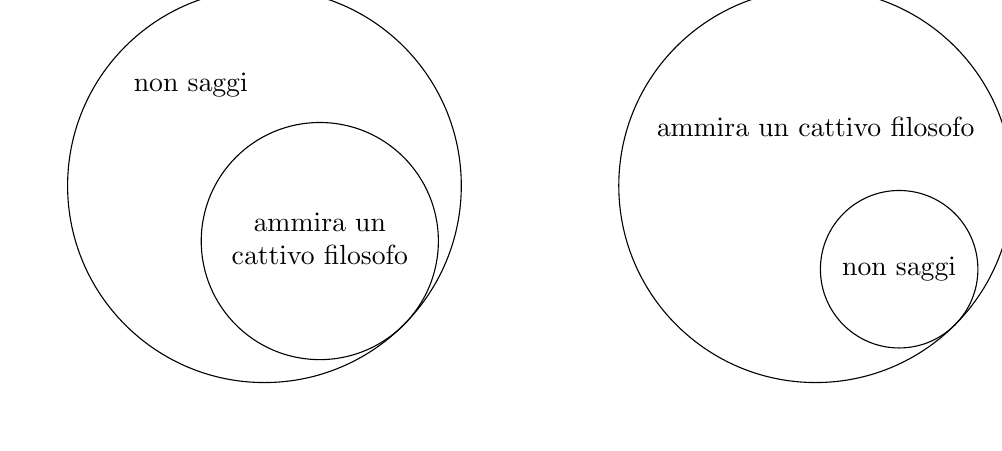
\begin{tikzpicture}

    \node
        [ circle,
            draw,
            minimum width=5cm,
            label={[label distance=-1.5cm]95:non saggi},
        ] (X) [xshift=1cm] {};

    \node
        [ circle,
            draw,
            minimum width=2cm,
            anchor=south east,
        ] (Y) at (X.south east) {$\begin{array}{c}\text{ammira un}\\ \text{cattivo filosofo}\end{array}$};

    \node
        [ circle,
            draw,
            minimum width=5cm,
            label={[label distance=-2cm]90:ammira un cattivo filosofo},
        ] (X1) [xshift=8cm] {};

    \node
        [ circle,
            draw,
            minimum width=2cm,
            anchor=south east,
        ] (Y1) at (X1.south east) {non saggi};


\end{tikzpicture}
\\
\noindent In quello di destra osserviamo che ci sono delle persone sagge (ovvero nel complementare dell'insieme dei non saggi) che ammirano cattivi filosofi, dunque in tale situazioni non solo i non saggi ammirano qualche cattivo filosofo, ma anche alcuni saggi. Dobbiamo dunque formalizzare la situazione a sinistra, ovvero che l'insieme degli ammiratori di cattivi filosofi � contenuto in quello delle persone non sagge.\\

\noindent La frase \lq\lq i buoni filosofi sono saggi\rq\rq\ si formalizza come
\[
\forall x (BF(x)\Rightarrow S(x)).
\]
La frase \lq\lq Aldo non ammira alcun filosofo\rq\rq\ si formalizza come
\[
\forall x (F(x)\Rightarrow \neg AM(a,x)).
\]
Infine la frase \lq\lq non tutti i filosofi sono buoni filosofi\rq\rq\ (che � la congettura del problema) si formalizza come
\[
\exists x (F(x)\wedge \neg BF(x)).
\]

\newpage

\noindent In Spass il problema si formalizza cos�:

\begin{verbatim}
begin_problem(laboratorio24072014).

list_of_descriptions.
name({*laboratorio24072014*}).
author({**}).
status(unsatisfiable).
description({**}).
end_of_list.

list_of_symbols.
  functions[(a,0)].
  predicates[(F,1),(BF,1),(S,1),(AM,2)].
end_of_list.

list_of_formulae(axioms).
formula(forall([x],implies(BF(x),F(x)))).
formula(exists([x],and(F(x),AM(x,a)))).
formula(forall([x,y],implies(and(S(x),BF(y)),AM(x,y)))).
formula(forall([x],implies(exists([y],and(AM(x,y),not(BF(y)))),not(S(x))))).
formula(forall([x],implies(F(x),not(AM(a,x))))).
formula(forall([x],implies(BF(x),S(x)))).
end_of_list.

list_of_formulae(conjectures).
formula(exists([x],and(F(x),not(BF(x))))).
end_of_list.

list_of_settings(SPASS).
{*
set_flag(DocProof,1).
*}
end_of_list.

end_problem.
\end{verbatim}

\noindent che produce il seguente output:

\begin{verbatim}
--------------------------SPASS-START-----------------------------
Input Problem:
1[0:Inp] ||  -> F(skc1)*.
2[0:Inp] ||  -> AM(skc1,a)*.
3[0:Inp] || BF(U) -> S(U)*.
4[0:Inp] || BF(U)* -> F(U).
5[0:Inp] || F(U) -> BF(U)*.
6[0:Inp] || AM(a,U)* F(U) -> .
7[0:Inp] || S(U) AM(U,V)* -> BF(V).
8[0:Inp] || BF(U) S(V) -> AM(V,U)*.
 This is a first-order Horn problem without equality.
 This is a problem that has, if any, a finite domain model.
 There are no function symbols.
 This is a problem that contains sort information.
 Axiom clauses: 7 Conjecture clauses: 1
 Inferences: IEmS=1 ISoR=1 IORe=1
 Reductions: RFMRR=1 RBMRR=1 RObv=1 RUnC=1 RTaut=1 
 RSST=1 RSSi=1 RFSub=1 RBSub=1 RCon=1
 Extras    : Input Saturation, Always Selection, No Splitting, Full Reduction,
 Ratio: 5, FuncWeight: 1, VarWeight: 1
 Precedence: div > id > AM > S > BF > F > a > skc0 > skc1
 Ordering  : KBO
Processed Problem:

Worked Off Clauses:

Usable Clauses:
1[0:Inp] ||  -> F(skc1)*.
9[0:Res:1.0,5.0] ||  -> BF(skc1)*.
2[0:Inp] ||  -> AM(skc1,a)*.
3[0:Inp] BF(U) ||  -> S(U)*.
4[0:Inp] BF(U) ||  -> F(U)*.
5[0:Inp] F(U) ||  -> BF(U)*.
6[0:Inp] F(U) || AM(a,U)* -> .
8[0:Inp] S(U) BF(V) ||  -> AM(U,V)*.
7[0:Inp] S(U) || AM(U,V)* -> BF(V).
	Given clause: 1[0:Inp] ||  -> F(skc1)*.
	Given clause: 9[0:Res:1.0,5.0] ||  -> BF(skc1)*.
	Given clause: 2[0:Inp] ||  -> AM(skc1,a)*.
	Given clause: 3[0:Inp] BF(U) ||  -> S(U)*.
	Given clause: 4[0:Inp] BF(U) ||  -> F(U)*.
	Given clause: 5[0:Inp] F(U) ||  -> BF(U)*.
	Given clause: 6[0:Inp] F(U) || AM(a,U)*+ -> .
	Given clause: 8[0:Inp] S(U) BF(V) ||  -> AM(U,V)*.
	Given clause: 17[0:SSi:16.1,5.1] S(a) F(U) ||  -> .
	Given clause: 7[0:Inp] S(U) || AM(U,V)*+ -> BF(V).
SPASS V 3.0
SPASS beiseite: Proof found.
Problem: /tmp/webspass-webform_2014-07-25_12:01:37_11886l.txt
SPASS derived 6 clauses, backtracked 0 clauses and kept 13 clauses.
SPASS allocated 587 KBytes.
SPASS spent	0:00:00.01 on the problem.
		0:00:00.00 for the input.
		0:00:00.00 for the FLOTTER CNF translation.
		0:00:00.00 for inferences.
		0:00:00.00 for the backtracking.
		0:00:00.00 for the reduction.


Here is a proof with depth 2, length 15 :
1[0:Inp] ||  -> F(skc1)*.
2[0:Inp] ||  -> AM(skc1,a)*.
3[0:Inp] BF(U) ||  -> S(U)*.
5[0:Inp] F(U) ||  -> BF(U)*.
6[0:Inp] F(U) || AM(a,U)*+ -> .
7[0:Inp] S(U) || AM(U,V)*+ -> BF(V).
8[0:Inp] S(U) BF(V) ||  -> AM(U,V)*.
9[0:Res:1.0,5.0] ||  -> BF(skc1)*.
16[0:Res:8.2,6.1] S(a) BF(U) F(U) ||  -> .
17[0:SSi:16.1,5.1] S(a) F(U) ||  -> .
18[0:SoR:17.0,3.1] F(U) BF(a) ||  -> .
19[0:Res:2.0,7.1] S(skc1) ||  -> BF(a)*.
21[0:SSi:19.0,1.1,9.0,3.0] ||  -> BF(a)*.
22[0:MRR:18.1,21.0] F(U) ||  -> .
23[0:UnC:22.0,1.0] ||  -> .
Formulae used in the proof : axiom1 axiom5 conjecture0 axiom4 axiom3 axiom2

--------------------------SPASS-STOP------------------------------
\end{verbatim}
\noindent che prova la correttezza della congettura.

\end{document}
